\documentclass{article}
\usepackage[utf8]{inputenc}
\usepackage[english]{babel}
\usepackage[T1]{fontenc}
\usepackage{csquotes}

%%% functional packages
\usepackage{amsmath, amssymb, amsthm, mathtools, mathrsfs}
\usepackage{physics, siunitx}
\usepackage{subcaption}     % for \subfigure
\usepackage{suffix}         % for \WithSuffix
\usepackage{multirow}
\usepackage{xspace}
\usepackage{comment}
\usepackage{graphicx}
\usepackage{algorithm}
\usepackage[noend]{algpseudocode}
\graphicspath{{_pics/}}

%%% configuration packages
\usepackage{titlesec}       % for \sectionbreak
\usepackage{authblk}        % for authors affiliations
\usepackage{fullpage}
\usepackage{enumitem}       % for configuration of enumerates

\usepackage[
    colorlinks
]{hyperref}

\usepackage[
    backend=biber,
    style=numeric,
    sorting=none,
    maxbibnames=99, minbibnames=99,
    natbib=true,
    doi=true,
    pagetracker,
    giveninits
]{biblatex}
\bibliography{tfd-slm}

%%% general aliases
\newcommand{\tran}{\mathsf{T}} %{^{\mkern-1.5mu\mathsf{T}}}

%%% \myoverbrace command (requires `xparse` package)
\NewDocumentCommand{\myoverbracetext}{m}{\text{#1}\\} % for internal use
\NewDocumentCommand\myoverbrace{ O{\int} m >{\SplitList{\\}}m }
{% two mandatory arguments: 2 - formula and 3 - caption delimited by \\
    \overbrace{\vphantom{#1}#2}^{\substack{\ProcessList{#3}{\myoverbracetext}}}
}

%%% material derivative (requires `suffix` package)
\newcommand\Dv[2][]{\frac{\mathrm{D}#1}{\mathrm{D}#2}}
\WithSuffix\newcommand\Dv*[2][]{\mathrm{D}#1/\mathrm{D}#2}

%%% problem-specific aliases
\newcommand{\fusion}[1]{{#1}_\mathrm{fus}}
\newcommand{\evapor}[1]{{#1}_\mathrm{vap}}
\newcommand{\OpenFOAM}{OpenFOAM\textregistered\xspace}

%%% bold symbols
\newcommand{\bv}{\vb{v}}
\newcommand{\bn}{\vu{n}}
\newcommand{\bx}{\vb{x}}
\newcommand{\btau}{\vb*\tau}
\newcommand{\matr}[1]{\vb{#1}} %{\mathbfit{#1}}

%%% for algorithms
\newcommand{\intCell}{\int_{V_p} \dd{V}}
\newcommand{\intFaces}{\oint_{\partial V_p} \dd{\vb*{s}}}

%%% for coloring
\usepackage{xcolor}
%\newcommand{\alert}[1]{\textcolor{red}{\bf #1}}
\newcommand{\alert}[1]{\textcolor{red}{#1}} % for highlighting
\newcommand{\oleg}[1]{\textcolor{magenta}{\footnote{\textcolor{magenta}{Oleg: #1}}}} % Oleg's remarks
\newcommand{\aslan}[1]{\textcolor{blue}{\footnote{\textcolor{blue}{Aslan: #1}}}} % Aslan's remarks

\title{Modeling and simulation of the melt-pool dynamics in laser powder-bed additive manufacturing}
\author{Oleg A. Rogozin}
\author{Aslan R. Kasimov}
\affil{Center for Design, Manufacturing and Materials \\
    Skolkovo Institute of Science and Technology, Moscow, Russia}
% \affil[2]{Dorodnicyn Computing Center,
%     Federal Research Center "Computer Science and Control" of Russian Academy of Science, Moscow, Russia}
\renewcommand\Affilfont{\itshape\small}
\date{}

\begin{document}

\maketitle

\begin{abstract}
%%% Aim
In this work, we investigate numerically the dynamics of the melt pool that forms in the laser powder-bed fusion process in additive manufacturing. The governing system of three-dimensional three-phase fluid dynamics equations  includes a wide range of physical effects such as: surface-tension with Marangoni stresses, evaporation of the melt, solidification, and temperature dependence of various fluid properties.
%
%%% Assumptions
All three phases are modeled as incompressible viscous heat-conducting fluids. The powder bed is treated as a set of individual immobile particles. The solidification of the melt is assumed to take place over a homogenized mushy layer modeled as a porous medium.
%
%%% Implementation and validation
The proposed thermo-fluid-dynamic model is implemented in an \OpenFOAM environment and is validated against experimental data on single tracks printed on an industrial 3D printer using 316L stainless steel powder.
Excellent\oleg{We sincerely hope so.} agreement is found with respect to the form and dimensions of the solidified track. The role of various physical effects that are included in the model is analyzed and their importance is discussed.
\end{abstract}

\tableofcontents

\subsection{Possible journals}
\begin{enumerate}
    \item Acta Materialia, Q1, SJR 3.76
    \item Additive Manufacturing, Q1, SJR 2.59
    \item Computational Materials, Q1, SJR 3.46
    \item Computational Materials Science, Q1/Q2, SJR 0.81
    \item Computers and Mathematics with Applications, Q1, SJR 1.00
    \item Journal of Materials Processing Technology, Q1, SJR 1.72
    \item International Journal of Advanced Manufacturing Technology, Q1, SJR 0.99
    \item Materials \& Design, Q1, SJR 1.95
\end{enumerate}

\subsection{TODO list}
\begin{enumerate}
    \item Ray-tracing algorithms~\cite{cook2019simulation}.
    \item Change of density in solid--liquid phase transition and shrinkage due to the density change as a function of temperature~\cite{wei2017thermal}.
    \item Powder particle packing (PPP) algorithm based on rain model~\cite{attar2011simulation}.
    \item Since $\Re>\num{e3}$ in some cases, turbulent viscosity for gas flow~\cite{zhirnov2018evaporation,gusarov2020entrainment,matthews2016denudation}.
    \item Multi-layer algorithm~\cite{attar2011simulation}.
\end{enumerate}

\section{Introduction}

Fluid-dynamics of the melt pool is the crucial physical process
for predicting the resulting properties of a printed part.
Powder-scale simulations help to understand the inherent instabilities of the melt pool
that determine the geometry of the solidified track.
In turn, this affects the uniformity of the printing and, very likely, the details of the grain formation
and the residual stresses in the printed part.
Furthermore, the melt-pool dynamics is expected to strongly influence the solidification-front evolution
and structure via local temperature gradients, which are coupled to the fluid flow.
A detailed exploration of these processes is a significant challenge for modeling
that should be undertaken in a follow-up work.

\section{Mathematical model}

%%% Assumptions of the model
The physical model employed in our study is subject to the following assumptions:
\begin{itemize}
    \item Gas, liquid, and solid are incompressible fluids with constant densities.
    \item Laser radiation is absorbed uniformly over the surface with a constant absorptivity, regardless of the angle of incidence.
    \item Solid media are at rest.
    \item The liquid behaviour is Newtonian with Arrhenius temperature dependence.
    \item The solidification interface is modeled as a mushy layer.
\end{itemize}
The last assumption allows us to model the solidification front structure as a porous medium
with a given permeability and to avoid computing the multi-scale complex structure
of the solidification front dynamics at the present level of modeling.
The following physical phenomena are described by the model:
\begin{itemize}
    \item Surface tension and thermal Marangoni effect.
    \item Solidification and evaporation of the molten metal.
    \item Recoil pressure and evaporative cooling (very important to suppress superheating).
    \item Radiative (thermal and laser) and convective heat transfer.
\end{itemize}

Moreover, the following physical effects are neglected:
\begin{itemize}
    \item Viscous heat dissipation.\oleg{I suggest to include now. Moreover, probably turbulent heat dissipation.}
    \item Wetting force.
    \item Chemical Marangoni effect.
    \item Optics, including absorption of the reflected laser radiation, shadow effects, and beam divergence.
    \item Shrinkage due to the density change as a function of temperature and phase transition.
    \item Kinetic energy of fluid flow.
    \item Vapour mass losses.
    \item Mechanical stresses in solid body.
\end{itemize}
Finally, some minor assumptions:
\begin{itemize}
    \item The laser beam has a Gaussian spatial distribution.
    \item Heat capacity and thermal conductivity are linear functions of temperature.
    \item The densities of liquid and solid metal are equal to each other.
    \item Viscosity of the gas does not depend on temperature.
    \item Enthalpy of evaporation does not depend on temperature.
\end{itemize}

%%% Three phases
Three phase states considered are given as
\begin{enumerate}[label=\arabic*)]
    \item gas: $\alpha=1$, $0\leq\phi\leq1$;
    \item liquid: $\alpha=0$, $\phi=1$;
    \item solid: $\alpha=0$, $\phi=0$.
\end{enumerate}

The principal scheme is shown in Fig.~\ref{fig:scheme}.
\oleg{I believe that it should be removed from the manuscript.}
\begin{figure}
    \centering
    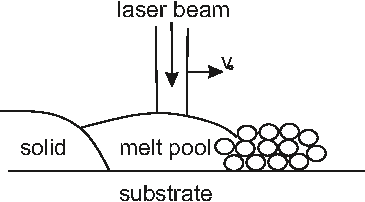
\includegraphics[width = 0.5\textwidth]{scheme}
    \caption{
        Schematics of laser powder-bed fusion.
    }\label{fig:scheme}
\end{figure}

%%% Governing equations
The governing equations for the gas fraction $\alpha$, density $\rho$, velocity $\bv$, and enthalpy $h$ are as follows:
\begin{gather}
    \pdv{\alpha}{t} + \bv\vdot\grad\alpha = 0, \label{eq:alpha}\\
    \div\bv = 0, \label{eq:continuity}\\
    \begin{multlined}
    \rho\pdv{\bv}{t} + \rho(\bv\vdot\grad)\bv =
        - \myoverbrace{K(1-\alpha)\frac{(1-\phi)^2}{\phi^3}\bv}
            {Darcy force with\\Kozeny--Carman\\permeability}
        + \myoverbrace{\div\btau}{viscous\\force}
        - \myoverbrace{\grad{p}}{pressure\\force}
        + \myoverbrace{\rho\vb{g}}{gravity\\force}
        - \myoverbrace{\rho\vb{g}\beta(T-T_0)}{buoyancy\\force}\\
        - \myoverbrace{\gamma\qty(\div\bn)\grad\alpha}{surface tension}
        + \myoverbrace{\dv{\gamma}{T}\qty(\bn\cp\grad{T}\cp\bn)|\grad\alpha|}{Marangoni force}
        -\myoverbrace{\frac{3-\evapor{a}}4\evapor{p}\grad\alpha}{recoil pressure}
    \end{multlined}\label{eq:v}\\
    \begin{multlined}
    \rho\pdv{h}{t} + \rho(\bv\vdot\grad)h
        = \myoverbrace[\qty(\frac12)^2]{\div(k\grad{T})}{heat conduction}
        + \myoverbrace{\frac{2AP}{\pi R_0^2}
            \exp\qty(-2\frac{\qty|(\bx-\bx_0)\cp\bn_0|^2}{R_0^2})|\grad\alpha|}{laser heat}\\
        - \myoverbrace{\epsilon\sigma\qty(T^4-T_0^4)|\grad\alpha|}{radiative cooling}
        - \myoverbrace{\frac{\evapor{a}\evapor{p}\evapor{h}}
            {(2\pi RT/M)^{1/2}}|\grad\alpha|}{evaporative cooling},
    \end{multlined}\label{eq:h}
\end{gather}
where $\rho$ is the density, $\bv$ is the velocity, $T$ is the temperature,
$p$ is the pressure, $\alpha$ is the gas fraction,
$(1-\alpha)\phi$ is the volume fraction of the molten metal,
$K>0$ is the coefficient related to permeability of the mushy layer,
$\gamma$ is the surface tension,
$\bn = \grad\alpha/|\grad\alpha|$ is the unit normal vector,
$\bn_0 = (0,0,1)$ specifies the direction of the laser beam,
$\vb{g}$ is the gravitational acceleration,
$\beta$ is the volume thermal expansion coefficient,
$k$ is the thermal conductivity, $A$ is the absorptivity of laser radiation, $P$ is the laser power,
$\bx_0$ is the coordinate of the laser focal point, $R_0$ is the radius of the laser beam,
$\epsilon$ is the emissivity,
$\sigma=\SI{5.67e-8}{W.m^{-2}.K^{-4}}$ is the Stefan--Boltzmann constant,
$T_0$ is the ambient temperature,
$0 < \evapor{a} < 1$ is the evaporation coefficient,
$\evapor{h}$ is the enthalpy of vaporization,
$M$ is the molar mass of the alloy,
$R = \SI{8.3145}{J.mol^{-1}.K^{-1}}$ is the gas constant.
Specific enthalpy $h$, viscous stress tensor $\btau$,
vapor pressure $\evapor{p}$,
and liquid fraction $\phi$ are calculated as follows:
\begin{gather}
    h = \int_0^T c_p(\xi)\dd{\xi} + (1-\alpha)\fusion{h}\phi(h), \label{eq:T}\\
    \btau = \mu\qty(\grad\bv + \qty(\grad\bv)^\tran), \label{eq:tau}\\
    \evapor{p}(T) = p_0\exp\qty(\frac{M\evapor{h}}{R}\qty(\frac1{T_B}-\frac1{T})), \label{eq:p_evapor}\\
    \phi(h) = \frac{1 + \tanh\qty(2\phi'_0(h-h_0))}2, \quad
        \phi'_0 = \frac1{h_L-h_S}, \quad h_0 = \frac{h_L+h_S}2, \label{eq:phi}
\end{gather}
where $c_p$ is the heat capacity,
$\fusion{h}$ is the enthalpy of fusion, $\mu$ is the viscosity, 
$p_0$ is the ambient pressure, $T_B$ is the boiling temperature,
$h_{S,L}$ are the enthalpy of solidus and liquidus, respectively.

%%% Material properties
All material properties $f = \rho, \mu, c_p, k$ are generally calculated as linear interpolations:
\begin{equation}\label{eq:properties}
    f = f_G\alpha + \qty[f_L\phi + f_S(1-\phi)](1-\alpha),
\end{equation}
where $f_S$, $f_L$, and $f_G$ correspond to the solid, liquid, and gas properties.
Specifically, the following expressions are used:
\begin{gather}
    \rho = \rho_G\alpha + \rho_L(1-\alpha), \label{eq:rho}\\
    \beta = \beta_G\alpha + \beta_L(1-\alpha), \label{eq:beta}\\
    \mu = \mu_G\alpha + \mu_L(1-\alpha), \quad 
        \mu_L = \mu_{L0}\exp\qty( \frac{E_a}{R} \qty(\frac1{T}-\frac1{T_l}) ), \label{eq:mu}\\
    c_p = c_{pG}\alpha + \qty[c_{pL}(T)\phi + c_{pS}(T)(1-\phi)](1-\alpha), \label{eq:c_p}\\
    k = k_G\alpha + \qty[k_L(T)\phi + k_S(T)(1-\phi)](1-\alpha), \label{eq:k}
\end{gather}
where all symbols with subscripts ${}_{S/L/G}$ are assumed to be constant,
$E_a$ is the activation energy.
The constant $K$ can be related to the viscosity and primary dendrite arm spacing $d_\text{PDAS}$~\cite{kubo1985mathematical}:
\begin{equation}\label{eq:permeability}
    K = \frac{180\mu_{L0}}{d_\text{PDAS}^2}.
\end{equation}
Relation~\eqref{eq:permeability} gives $K \approx \SI{e12}{kg.m^{-3}.s^{-1}}$ for ...,
but due to model smoothing of $\phi$, $K = \SI{e3}{kg.m^{-3}.s^{-1}}$ is chosen as a large enough numerical constant.

%This is of equations are similar to that used in~\cite{wang2019powder}.
The evaporation effects are described and critically analyzed in~\cite{cook2019simulation}, implemented in~\cite{khairallah2016laser}.

\subsection{Fidelity of the model}\oleg{I still do not know how to name this subsection}

\begin{enumerate}
    \item Why do we incorporate Marangoni, recoil pressure, evaporative/radiative cooling?
    \item Why do we employ the Darcy--Brinkman penalization?\cite{voller1987fixed, le2006interfacial} Kozeny--Carman permeability?
    \item Clausius--Clayperon~\cite{klassen2014evaporation, cook2019simulation}
\end{enumerate}

%%% Ray-tracing
% [Rogozin] which introduces concentrated on the powder surface in the shadow zone.
It will be remedied by introducing a more sophisticated ray-tracing algorithm
for a more accurate treatment of the laser-source interaction with the surface of the powder particles,
which is part of the future work.

\subsection{Dimensionless analysis}

Preliminary conclusions:
\begin{enumerate}
    \item $\Re$ number. The melt pool is in a laminar flow regime, while  turbulent flows can form in the ambient gas.
\end{enumerate}

\section{Numerical algorithms}

%%% Simulation environment
In all the cases considered further, the numerical implementation of the models is carried out
in the open-source environment \OpenFOAM, primarily based on the finite-volume method,
which allows for efficient and accurate solution of complex 3D problems of continuum physics,
including fluid dynamics, solid mechanics, and phase transitions within the framework of phase-field modeling.
The computing environment of \OpenFOAM is well-suited to these types of models,
and furthermore allows for adaptive meshes that are necessary
for resolving the multi-scale nature of the phenomena that take place.
For example, the solidification often proceeds via the formation of complex dendritic structures,
which must be resolved in simulations and which play an important role in the formation of grains in the solid part.

%%% Solver
The thermo-fluid-dynamic model is implemented as an extension of \verb+interFoam+ solver.
\verb+interFoam+ is the well established \OpenFOAM solver for multiphase flow
based on the volume-of-fluid (VOF) method for interface reconstruction.
The energy equation~\eqref{eq:h} is discretized as follows:
\begin{equation}\label{eq:h_scheme}
    \begin{aligned}
    \underbrace{
        \intCell \pdv{\rho h}{t}
    }_\text{implicit} &+ \underbrace{
        \intFaces \qty(\rho h\bv - \frac{k}{c_p}(1+\phi')\grad{h})
    }_\text{implicit} \\ &= \frac{2AP}{\pi R_0^2}\underbrace{
        \intCell |\grad\alpha\vdot\bn_0|\exp\qty[-2\frac{(x-x_0)^2 + (y-y_0)^2}{R_0^2}]
    }_\text{explicit}.
    \end{aligned}
\end{equation}

%%% Method of solution of PDE
The overall time-marching scheme is based on the classical PIMPLE algorithm
and is outlined in~\ref{alg:tfd}.

\begin{algorithm}[H]
\caption{Global solution procedure for the thermo-fluid-dynamic model}\label{alg:tfd}
\begin{algorithmic}[1]
    \Require values from previous time step $\alpha$, $\rho$, $\bv$, $p$, $h$, $T$.
    \State Set time step $\Delta{t}$ based on the Courant number
    \begin{equation}\label{eq:Courant}
        \mathrm{Co} = \max\qty( \rho\bv\frac{\Delta t}{\Delta x} ).
    \end{equation}
    \State Calculate $c_p$ and $k$ from $\phi$ and $T$ using~\eqref{eq:c_p} and~\eqref{eq:k}.
    \State Find $h$ as a solution of~\eqref{eq:h} using scheme~\eqref{eq:h_scheme}.
    \State Calculate $\phi$ and $T$ from $h$ using~\eqref{eq:phi} and~\eqref{eq:T}.
    \While{not converged (outer correction loop)}
        \State Find $\alpha$ as a solution of~\eqref{eq:alpha} using a VOF scheme.
        \State Calculate $\rho$ and $\mu$ from~\eqref{eq:rho} and~\eqref{eq:mu}.
        \While{not converged (pressure correction loop)}
            \State Find $p$ as a solution of the Poisson equation derived by substituting~\eqref{eq:continuity}
            into the divergence of~\eqref{eq:v}.
            \State Calculate $\bv$ from the explicit discretization of~\eqref{eq:v} using the updated $p$.
        \EndWhile
    \EndWhile
\end{algorithmic}
\end{algorithm}

\section{Verification}

--- We are going to present a set of verification tests for each term of equations. See Chapter 4 in~\cite{attar2011simulation}.

\section{Results and discussion}

\begin{table}
    \centering
    \caption{Material properties of stainless steel 316L used for numerical simulations}
    \label{table:ss316l}
    \begin{tabular}{lcccc}
        \hline\noalign{\smallskip}
        Physical property & Symbol & Value & Unit & Reference \\[3pt] \hline\noalign{\smallskip}
        \multirow{2}*{Viscosity} & $\mu_G$ & \num{1.5e-5} & \multirow{2}*{\si{Pa.s}} &  \\
        & $\mu_L$ & $\num{6.759e-3}\exp(\SI{45.6}{kJ/mol}/RT)$ & & \cite{kim1975thermophysical} \\[3pt]
        \noalign{\smallskip}
        \multirow{2}*{Density} & $\rho_G$ & \num{1} & \multirow{2}*{\si{kg.m^{-3}}} & \\
        & $\rho_L$ & \num{6966} & & \\[3pt]
        \noalign{\smallskip}
        \multirow{2}*{Thermal expansion} & $\beta_G$ & \num{0} & \multirow{2}*{\si{K^{-1}}} & \\
        & $\beta_L$ & \num{0} & & \\[3pt]
        \noalign{\smallskip}
        \multirow{3}*{Thermal conductivity} & $k_G$ & \num{0.2} & \multirow{3}*{\si{W.m^{-1}.K^{-1}}} & \\
        & $k_L$ & $\num{12.41} + \SI{3.279e-3}{K^{-1}}T $ & & \cite{kim1975thermophysical} \\
        & $k_S$ & $\num{9.248} + \SI{1.571e-2}{K^{-1}}T $ & & \cite{kim1975thermophysical} \\[3pt]
        \noalign{\smallskip}
        \multirow{3}*{Heat capacity} & $c_{pG}$ & \num{1006} & \multirow{3}*{\si{J.kg^{-1}.K^{-1}}} & \\
        & $c_{pL}$ & $\num{769.9}$ & & \cite{kim1975thermophysical} \\
        & $c_{pS}$ & $\num{459.0} + \SI{0.1328}{K^{-1}}T $ & & \cite{kim1975thermophysical} \\[3pt]
        \noalign{\smallskip}
        Enthalpy of fusion & $\fusion{h}$ & \num{268} & \multirow{2}*{\si{kJ.kg^{-1}}} & \\
        Enthalpy of evaporation & $\evapor{h}$ & \num{7410} & & \\[3pt]
        \noalign{\smallskip}
        Solidus & $T_S$ & \num{1648} & \multirow{3}*{\si{K}} & \\
        Liquidus & $T_L$ & \num{1673} & & \\
        Boiling temperature & $T_B$ & \num{3086} & & \\[3pt]
        \noalign{\smallskip}
        Surface tension & $\gamma$ & $\num{3.282} - \SI{8.9e-4}{K^{-1}}T$ & \si{kg.s^{-2}} & \cite{khairallah2016laser} \\[3pt]
        \noalign{\smallskip}
        Absorptivity & $A$ & \num{0.3} & \multirow{3}*{ } & \\
        Emissivity & $\epsilon$ & \num{0.3} & & \\
        Evaporation coefficient & $\evapor{a}$ & \num{0.82} & & \\[3pt]
        \hline
    \end{tabular}
\end{table}

The material properties for SS316L are presented in Fig.~\ref{table:ss316l}.
The values of absorptivity and emissivity are taken as for nonoxidized metal surface,
since we assume that selective laser melting take place in argon inert atmosphere.

\subsection{Single tracks}

Parametric study for various printing regimes.
\begin{enumerate}
    \item flat melt pool
    \item unstable key hole
    \item developed key hole
\end{enumerate}

\subsection{Validation experiments}

\begin{itemize}
    \item Trumpf TruPrint 1000
    \item how was polished, etched, microscope
\end{itemize}


\begin{enumerate}
    \item Cross sections.
    \item Several longitudinal sections for each track.
\end{enumerate}

\section{Conclusions}

%%% What have we done?
Within the framework of this formulation, we have validated the model with a single-track problem
for the powder-bed fusion of SS316L and have found an excellent agreement with experimental data
with respect to the form and dimensions of the solidified track in its cross section.

\section{Acknowledgements}
To Denis Firsov and Yulia Kuzminova for helping in preparing experimental results.
To Diana Gazizova for helping in data processing and fruitful discussions.
To Stanislav Evlashin, Svyatoslav Chugunov, Igor Shishkovsky, Michail Perevozchikov, and Iskander Akhatov for valuable discussions.

\appendix

\section{Multi-domain formulation}

%%% Governing equations
In the sharp-interface limit, the single-domain governing equations for $\Omega=\Omega_G\cup\Omega_L\cup\Omega_S$ can be regularized and decomposed as follows: 
\begin{equation}
    \div\bv_g = 0, \quad
    \rho_G\Dv[\bv_g]{t} = \mu_G\laplacian\bv_g - \grad{p_g} + \rho_G\vb{g}(1-\beta_G(T-T_0)), \quad
    \rho_G\Dv[h_g]{t} = \frac{k_G}{c_{pG}}\laplacian{h_g} 
\end{equation}
for $\bv_g$, $p_g$, and $h_g$ in the gas domain $\Omega_G$;
\begin{equation}
    \div\bv_l = 0, \quad
    \rho_L\Dv[\bv_l]{t} = \div\btau_L - \grad{p_l} + \rho_L\vb{g}(1-\beta_L(T-T_0)), \quad
    \rho_L\Dv[h_l]{t} = \div(\frac{k_L}{c_{pL}}\grad{h_l})
\end{equation}
for $\bv_l$, $p_l$, and $h_l$ in the liquid domain $\Omega_L$; and
\begin{equation}
    \bv_s = 0, \quad \rho_S\pdv{h_s}{t} = \div(\frac{k_S}{c_{pS}}\grad{h_s})
\end{equation}
for $\bv_s$ and $h_s$ in the solid domain $\Omega_S$.
Here, $\Dv*{t} = \pdv*{t} + \bv\vdot\grad$ is the material derivative.

%%% Boundary conditions
The interfacial boundary conditions take the following form:
\begin{gather}
    \bv_g = \bv_{LG} = \bv_l, \quad T_g = T_{LG} = T_l, \quad v_{LG} = \bv_g\vdot\bn_{LG}, \\
    \qty(p_g - p_l + \gamma\div\bn_{LG} + \frac{3-\evapor{a}}4\evapor{p}(T_{LG}))\bn_{LG}
    = (\btau_G - \btau_L)\vdot\bn_{LG} + \dv{\gamma}{T}\grad{T_{LG}}, \\
    \begin{aligned}
    \qty( \frac{k_L}{c_{pL}}\grad{h}_l - \frac{k_G}{c_{pG}}\grad{h}_g )&\vdot\bn_{LG}
        = \frac{2AP}{\pi R_0^2}\exp(-2\frac{\abs{(\vb{x}-\vb{x_0})\cp\bn_0}^2}{R_0^2}) \\
        &- \epsilon\sigma\qty(T_{LG}^4-T_0^4)
        - \frac{\evapor{a}\evapor{p}(T_{LG})\evapor{h}}{(2\pi RT_{LG}/M)^{1/2}},
    \end{aligned}
\end{gather}
for the gas--liquid interface $\Omega_{GL} = \Omega_G\cap\Omega_L$,
which moves at the speed $v_{LG}$ along the unit normal $\bn_{LG}$ directed into the gas (coincides with $\bn$);
\begin{gather}
    \bv_g = 0, \quad T_g = T_s, \\
    \begin{aligned}
    \qty( \frac{k_S}{c_{pS}}\grad{h}_s - \frac{k_G}{c_{pG}}\grad{h}_g )&\vdot\bn_{SG}
        = \frac{2AP}{\pi R_0^2}\exp(-2\frac{\abs{(\vb{x}-\vb{x_0})\cp\bn_0}^2}{R_0^2}),
    \end{aligned}
\end{gather}
for the gas--solid interface $\Omega_{GS} = \Omega_G\cap\Omega_S$,
which moves at the speed $v_{SG}$ along the unit normal $\bn_{SG}$ directed into the gas; \begin{equation}
    \bv_l = 0, \quad h_l = h_L, \quad h_s = h_S, \quad
    \qty( \frac{k_S}{c_{pS}}\grad{h}_s - \frac{k_L}{c_{pL}}\grad{h}_l )\vdot\bn_{SL}
        = \rho_L(h_L - h_S)v_{SL}
\end{equation}
for the liquid--solid interface $\Omega_{LS} = \Omega_L\cap\Omega_S$,
which moves at the speed $v_{SL}$ along the unit normal $\bn_{SL}$ directed into the liquid. 
Note that both radiative and evaporative cooling are neglected at the gas--solid interface.

\printbibliography

\end{document}
